%! TEX root = ../000-main.tex
\chapter[NL dim. red.]{Nonlinear dimensionality reduction}

\section[Introduction]{Introduction to dimensionality reduction}
\paragraph{References:}
\cite[Chapter 8]{johnson_applied_2007},
\cite[Chapters 5 and 6]{pena_alisis_2002},
\cite[Section 11.1]{venables_exploratory_2002},
\cite[Sections 14.5.1, 14.8 and 14.9]{hastie_elements_2009}

We observe $n$ independent objects $\mathcal{O}_i,\;i=1,\ldots,n$ from a given population.

In general, they belong to a large-dimensional (or even infinite-dimensional) space $\Omega$.

\begin{definition}{Dimensionality reduction problem}{}
    We want to find a low dimensional configuration $\boldsymbol{Y}$, that is an
    $n \times q$ matrix, where $q < n$ such that each of its rows $\boldsymbol{y}_i$ can
    be identified with the observed object $\mathcal{O}_i$ in some way:
    \begin{itemize}
        \item An application $\rho: \mathbb{R}^q \to \Omega$ such that
            $\rho(\boldsymbol{y}_i) \approxeq \mathcal{O}_i,\quad i=1,\ldots,n$.
        \item We can define a distance between $\boldsymbol{y}_i$ and $\boldsymbol{y}_j$,
            such that the distance between $\mathcal{O}_i$ and $\mathcal{O}_j$ is close
            to the dissimilarity between the observed objects $\mathcal{O}_i$ and
            $\mathcal{O}_j,\; \forall i,j \in \{1,\ldots,n\}$.
        \item \ldots
    \end{itemize}
    \begin{note}
        When dimensionality reduction is for visualization purposes, $q = 2$ is
        usually chosen.
    \end{note}
\end{definition}

\subsection{Two types of information from the observed objects}
We consider two different ways of extracting information from the observed objects:
\begin{itemize}
    \item Sampling information as a \iemph{data matrix} $\boldsymbol{X}$ of
        size $n \times p$ ($n$ individuals and $p$ attributes, $p \gg q$).
        \begin{itemize}
            \item Principal component analysis (PCA).
            \item Principal curves (Nonlinear version of PCA) \cite{hastie_principal_1989,delicado_another_2001}.
        \end{itemize}
    \item Sampling information as a distance matrix $\boldsymbol{D}$ of size
        $n \times n$.
        \begin{itemize}
            \item Multidimensional scaling (MDS).
            \item Local MDS
            \item Isometric mapping (ISOMAP, Nonlinear version of MDS).
            \item t-Stochastic Neighbor Embedding (t-SNE).
        \end{itemize}
\end{itemize}

\section[PCA]{Principal component analysis (PCA)}\index{PCA}

\begin{definition}{Principal component analysis (PCA)}{PCA}
    Multivariate analysis technique that intends to explain the
    \iemph{variance-covariance structure} through a few linear combinations of the original
    variables.

    \paragraph{Main goals:} Interpretation and dimensionality reduction.
\end{definition}

\begin{definition}{Variance-covariance structure}{}
    The variance-covariance structure of a random vector $\boldsymbol{X} \in \mathbb{R}^p$
    is defined as the $p \times p$ matrix $\boldsymbol{V} = \boldsymbol{V}(\boldsymbol{X})$
    such that:
    \begin{equation*}
        \boldsymbol{V}_{ij} = \mathrm{Cov}(X_i,X_j) = \mathrm{E}[(X_i - \mathrm{E}[X_i])(X_j - \mathrm{E}[X_j])].
    \end{equation*}
    \tcblower
    The variance is the diagonal of the variance-covariance matrix:
    \begin{equation*}
        \boldsymbol{\sigma}^2 = \mathrm{diag}(\boldsymbol{V}).
    \end{equation*}
\end{definition}

\subsubsection{Finding the first principal component (q=1)}
\begin{figure}[H]
    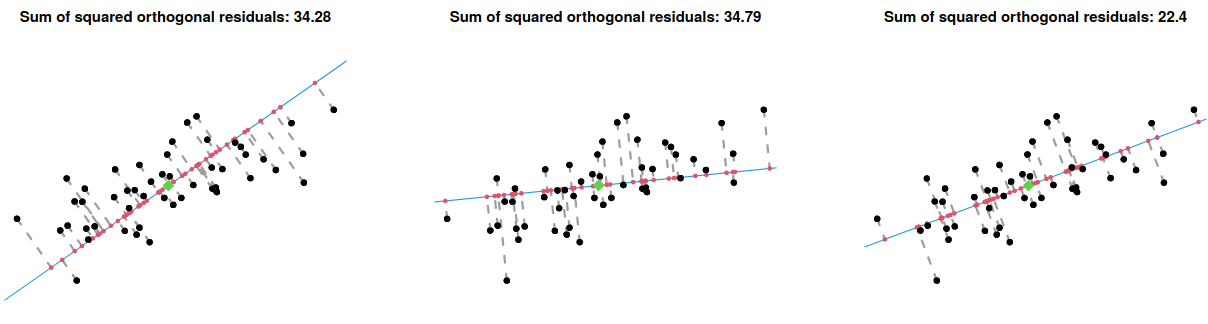
\includegraphics{pca_q1}
\end{figure}
We observe $\boldsymbol{x}_i \in \mathbb{R}^p,\;i=1,\ldots,n$ with mean $\boldsymbol{m}$.
For $\boldsymbol{a} \in \mathbb{R}^p,\, \lVert \boldsymbol a \rVert = 1$, the
projection vector of $(\boldsymbol{x} - \boldsymbol{m})$ in the direction of $\boldsymbol{a}$ is:
$P_{\boldsymbol{a}}(\boldsymbol{x} - \boldsymbol{m}) = \bigl( (\boldsymbol x - \boldsymbol m)' \boldsymbol a \bigr)
\boldsymbol{a}$. These two problems:
\begin{align*}
    \min_{\boldsymbol{a} \in \mathbb{R}^p,\, \lVert \boldsymbol a \rVert = 1} &\sum_{i=1}^n
        \left\lVert \boldsymbol{x}_i - \boldsymbol{m} - P_{\boldsymbol{a}}(\boldsymbol{x}_i - \boldsymbol{m}) \right\rVert^2 \tag{Minimizing the orthogonal residuals}\\
    \max_{\boldsymbol{a} \in \mathbb{R}^p,\, \lVert \boldsymbol a \rVert = 1} &\sum_{i=1}^n
        \left\lVert P_{\boldsymbol{a}}(\boldsymbol{x}_i - \boldsymbol{m}) \right\rVert^2
        \tag{Maximizing the inertia of the projected data}
\end{align*}
have the same solution $\boldsymbol{a}^*$, which we will call the \iemph{first principal component},
by Pythagoras' theorem:
\begin{equation*}
    \sum_{i=1}^n \left\lVert \boldsymbol{x}_i - \boldsymbol{m} \right\rVert^2
    = \sum_{i=1}^n \left\lVert
        \boldsymbol{x}_i - \boldsymbol{m} - P_{\boldsymbol{a}^*}(\boldsymbol{x}_i - \boldsymbol{m})
    \right\rVert^2
    + \sum_{i=1}^n \left\lVert P_{\boldsymbol{a}^*}(\boldsymbol{x}_i - \boldsymbol{m}) \right\rVert^2.
\end{equation*}

Let $\hat{V} = (\boldsymbol{v}_1,\ldots,\boldsymbol{v}_p)$ and $\hat{D} = \mathrm{Diag}(\hat{\lambda}_1,\ldots,\hat{\lambda}_p)$

Let $\boldsymbol S = \hat{V}\hat{D}\hat{V}'$ be the spectral decomposition of $\boldsymbol{S}$.

Then, the data matrix of sampling principal components is:
\begin{equation*}
    \boldsymbol{Y} = (\boldsymbol{y}_1,\ldots,\boldsymbol{y}_n) = (\boldsymbol{X} - \boldsymbol 1_n \boldsymbol m ')\hat{V}.
\end{equation*}
Roughly speaking, the sampling principal components are uncorrelated linear combinations of the
observed variables having the largest possible variability.

\begin{note}
    In this, way one of the two main goals of PCA is met: Interpretation.
\end{note}

\subsection{Single value decomposition (SVD)}

\begin{theorem}{Singular-Value Decomposition}{svd}
    Let $A$ be an $n \times p$ matrix. Then there exists an orthogonal matrix $U$ of size $n \times n$,
    and a orthogonal matrix $V$ of size $p \times p$ such that:
    \begin{equation*}
        A = U \Gamma V'
    \end{equation*}
    Where the $n \times p$ matrix $\Gamma$ has $(i,\, i)$ entry $\gamma_i \geq 0,\;i=1,\ldots,\min(n,p)$
    and the other entries are zero (diagonal matrix). The positive entries $\gamma_i$ are called
    the \iemph{singular values} of $A$. The number of singular values coincides with $k$, the rank of $A$.
    \tcblower
    \paragraph{Remark:} Let $\boldsymbol{u}_i$ be the columns of $U$ and let $\boldsymbol{v}_i'$ be the
    rows of $V'$. Then:
    \begin{equation*}
        A = U \Gamma V' = \sum_{i=1}^k \gamma_i \boldsymbol{u}_i \boldsymbol{v}_i'
    \end{equation*}
\end{theorem}

\subsubsection{SVD and PCA}

Let $A = \boldsymbol{X} - \boldsymbol 1_n \boldsymbol m '$. Then $A'A = (n - 1) \boldsymbol{S} =
(n - 1) \hat{V} \hat{D} \hat{V}'$.

Let $(\boldsymbol X - \boldsymbol 1_n \boldsymbol m ') = \hat{U}\Gamma \hat{V}'$ be SVD of $A$

$\boldsymbol{Y} = (\boldsymbol X - \boldsymbol 1_n \boldsymbol m ') \hat{V} \iff
\boldsymbol Y \hat{V}' = (\boldsymbol X - \boldsymbol 1_n \boldsymbol m ') = \hat{U}\Gamma\hat{V}'$,
then $\boldsymbol{Y} = \hat{U}\Gamma$.

The best approximation of rank $s$ to $A$ is:
\begin{equation*}
    \sum_{j=1}^s \gamma_j \boldsymbol{u}_j \boldsymbol{v}_j' = \sum_{j=1}^s \boldsymbol{y}_j \boldsymbol{v}_j' 
\end{equation*}
Therefore, the best approximation to $\boldsymbol{X}$ of rank $s$ is:
\begin{equation*}
    \boldsymbol{X} \approx \boldsymbol 1_n \boldsymbol m ' + \sum_{j=1}^s \boldsymbol{y}_j \boldsymbol{v}_j'
\end{equation*}
For the $i$-th row of $\boldsymbol{X}$:
\begin{equation*}
    \boldsymbol{x}_i \approx \boldsymbol{m} + \sum_{j=1}^s y_{ij} \boldsymbol{v}_j'
\end{equation*}
where $y_{ij}$ is the score of the $i$-th observation on the $j$-th principal component.

\begin{note}
    With this, the second goal of PCA is met: Dimensionality reduction.
\end{note}

\section{Multidimensional scaling (MDS)}

\begin{definition}{Multidimensional scaling (MDS)}{mds}\index{mds}
    is a dimensionality reduction technique based on \emph{inter-individual distances}.
\end{definition}

\begin{definition}{Euclidean configuration}{}
For $n$ individuals, let $\boldsymbol{D} = (\delta_{ij})$ be the $n \times n$ matrix of inter-individual
distances.

Assume that for a $q \leq n$ there exists a $n \times q$ data matrix $\boldsymbol{X}$ such that
the Euclidean distance between the $i$-th and $j$-th row of $\boldsymbol{X}$,
$\left\lVert \boldsymbol{x}_i - \boldsymbol{x}_j \right\rVert$, is equal to $\delta_{ij}$.

We say that $\boldsymbol{X}$ is a \iemph{Euclidean configuration} of $\boldsymbol{D}$.
\tcblower
\begin{note}
    Such configuration does not always exist.
\end{note}
\end{definition}

When it does exist, $\boldsymbol{D}$ is said to be Euclidean. In this
case $\boldsymbol{X}$ can be chosen verifying the following conditions:
\begin{itemize}
    \item It has orthogonal columns.
    \item For $1 \leq q \leq r$, the first $q$ columns of $\boldsymbol{X}$,
        $\boldsymbol{\tilde{X}}_a$, make up the $q$-dimensional configuration that
        best approximates the observed distances.
\end{itemize}
The columns of $\boldsymbol{X}$ are called \iemph{principal coordinates}.

When an Euclidean configuration does not exist, MDS allows to
obtain approximated solutions. That is, MDS looks for a $q$-dimensional
configuration $\boldsymbol{X}$ such that the Euclidean distances between
the rows of $\boldsymbol{X}$ are as close as possible to the observed
distances.

\subsection{Classical metric scaling}

If a $n \times p$ matrix $\boldsymbol{X}$ (with 0 mean by columns) is observed
and Euclidean distances are used, then: \emph{MDS and PCA give the same results}.

\subsection{Non-classical metric scaling}

Let $\boldsymbol{D} = (\delta_{ij})^n_{i,j=1}$ be the inter-individual distance
matrix recorded for the $n$ objects forming our sample.

Fix a tentative dimension $q$ and a $n \times q$ matrix $\boldsymbol{X}$.
Let $d_{ij} = \left\lVert \boldsymbol{x}_i - \boldsymbol{x}_j \right\rVert$ be the
Euclidean distance between the $i$-th and $j$-th row of $\boldsymbol{X}$.

The metric \iemph{STRESS} (STandardized REsidual Sum of Squares), a measure
of the relative error made when matrix $\boldsymbol{X}$ is considered as
an Euclidean configuration for the distance matrix $\boldsymbol{D}$, is defined as:
\begin{equation*}
    \text{STRESS}_M(\boldsymbol{D}, \boldsymbol{X}) = \sqrt{\frac
        {\sum_{i<j}(\delta_{ij} - d_{ij})^2}
        {\sum_{i<j}\delta_{ij}^2}
    }
\end{equation*}

The non-classical metric scaling problem is the following:
\begin{equation*}
    \min_{\boldsymbol{X} \in \mathds{R}^{n\times q}} \text{STRESS}_M(\boldsymbol{D}, \boldsymbol{X})
\end{equation*}

There is also S-STRESS:
\begin{equation*}
    \text{S-STRESS}_M(\boldsymbol{D}, \boldsymbol{X}) = \sqrt{\frac
        {\sum_{i<j}(\delta_{ij}^2 - d_{ij}^2)^2}
        {\sum_{i<j}\delta_{ij}^4}
    }
\end{equation*}

\subsection{Non-metric scaling}
Non-metric scaling uses only the ranks of the inter-individual distances $\delta_{ij}$.
The metric used is the Non-metric Stress (NMS):
\begin{equation*}
    \text{STRESS}_{NM}(\boldsymbol{D}, \boldsymbol{X}, f) = \sqrt{\frac
        {\sum_{i<j}(\text{rank}(\delta_{ij}) - d_{ij})^2}
        {\sum_{i<j}d_{ij}^2}
    }
\end{equation*}
Where $f: \mathds{R}^+ \to \mathds{R}^+$ is an increasing function.

The non-metric scaling problem is the following:
\begin{equation*}
    \min_{\boldsymbol{X} \in \mathds{R}^{n\times q}} \min_{f\uparrow} \text{STRESS}_{NM}(\boldsymbol{D}, \boldsymbol{X}, f)
\end{equation*}

\section{Distances and similarities}

\begin{definition}{Metric and Semi-metric}{metric}

    Let $\Omega$ be a set of objects. The application:
    \begin{equation*}
        d: \Omega \times \Omega \to \mathds{R}
    \end{equation*}
    is a \iemph{semi-metric} if it verifies the following properties $\forall P, Q, R \in \Omega$:
    \begin{align*}
        d(P, Q) &= d(Q, P) \tag{symmetry} \\
        d(P, Q) &\geq 0 \tag{non-negativity} \\
        d(P, P) &= 0 \tag{identity} \\
        d(P, Q) &\leq d(P, R) + d(R, Q) \tag{triangle inequality}
    \end{align*}

    \begin{marker}
        Additionally, if $d(P, Q) = 0 \implies P = Q$, then $d$ is a \iemph{metric} (or \emph{distance}).
    \end{marker}
\end{definition}

\begin{definition}{Similarity}{similarity}

    Let $\Omega$ be a set of objects. The application:
    \begin{equation*}
        s: \Omega \times \Omega \to \mathds{R}
    \end{equation*}
    is a \iemph{similarity} if it verifies the following properties $\forall P, Q, R \in \Omega$:
    \begin{align*}
        s(P, Q) &= s(Q, P) \tag{symmetry} \\
        s(P, Q) &\geq 0 \tag{non-negativity} \\
        s(P, P) &= s(Q, Q) \\
        s(P, Q) &\leq s(R, R)
    \end{align*}
    Additionally, it is required that $s(P, Q)$ is an increasing function of
    the proximity between $P$ and $Q$.
\end{definition}

\subsection{Similarities to and from distances}
\begin{equation*}
    s(P, Q) = \frac{1}{1 + d(P, Q)}
\end{equation*}

If the similarity function $s$ is a valid kernel function with $s(P, P) = 1,\;\forall P\in\Omega$,
and $s(P, Q) < 1,\;\forall P \neq Q \in \Omega$, then:
\begin{equation*}
    d(P, Q) = \sqrt{2\bigl(1 - s(P, Q)\bigr)}
\end{equation*}

% \section{Principal Curves}
% \section{Local MDS}
% \section{ISOMAP}
% \section{t-Stochastic Neighbor Embedding}
